\begin{figure}[ht!]
    \centering
    \begin{subfigure}{.3\textwidth}
        \centering
        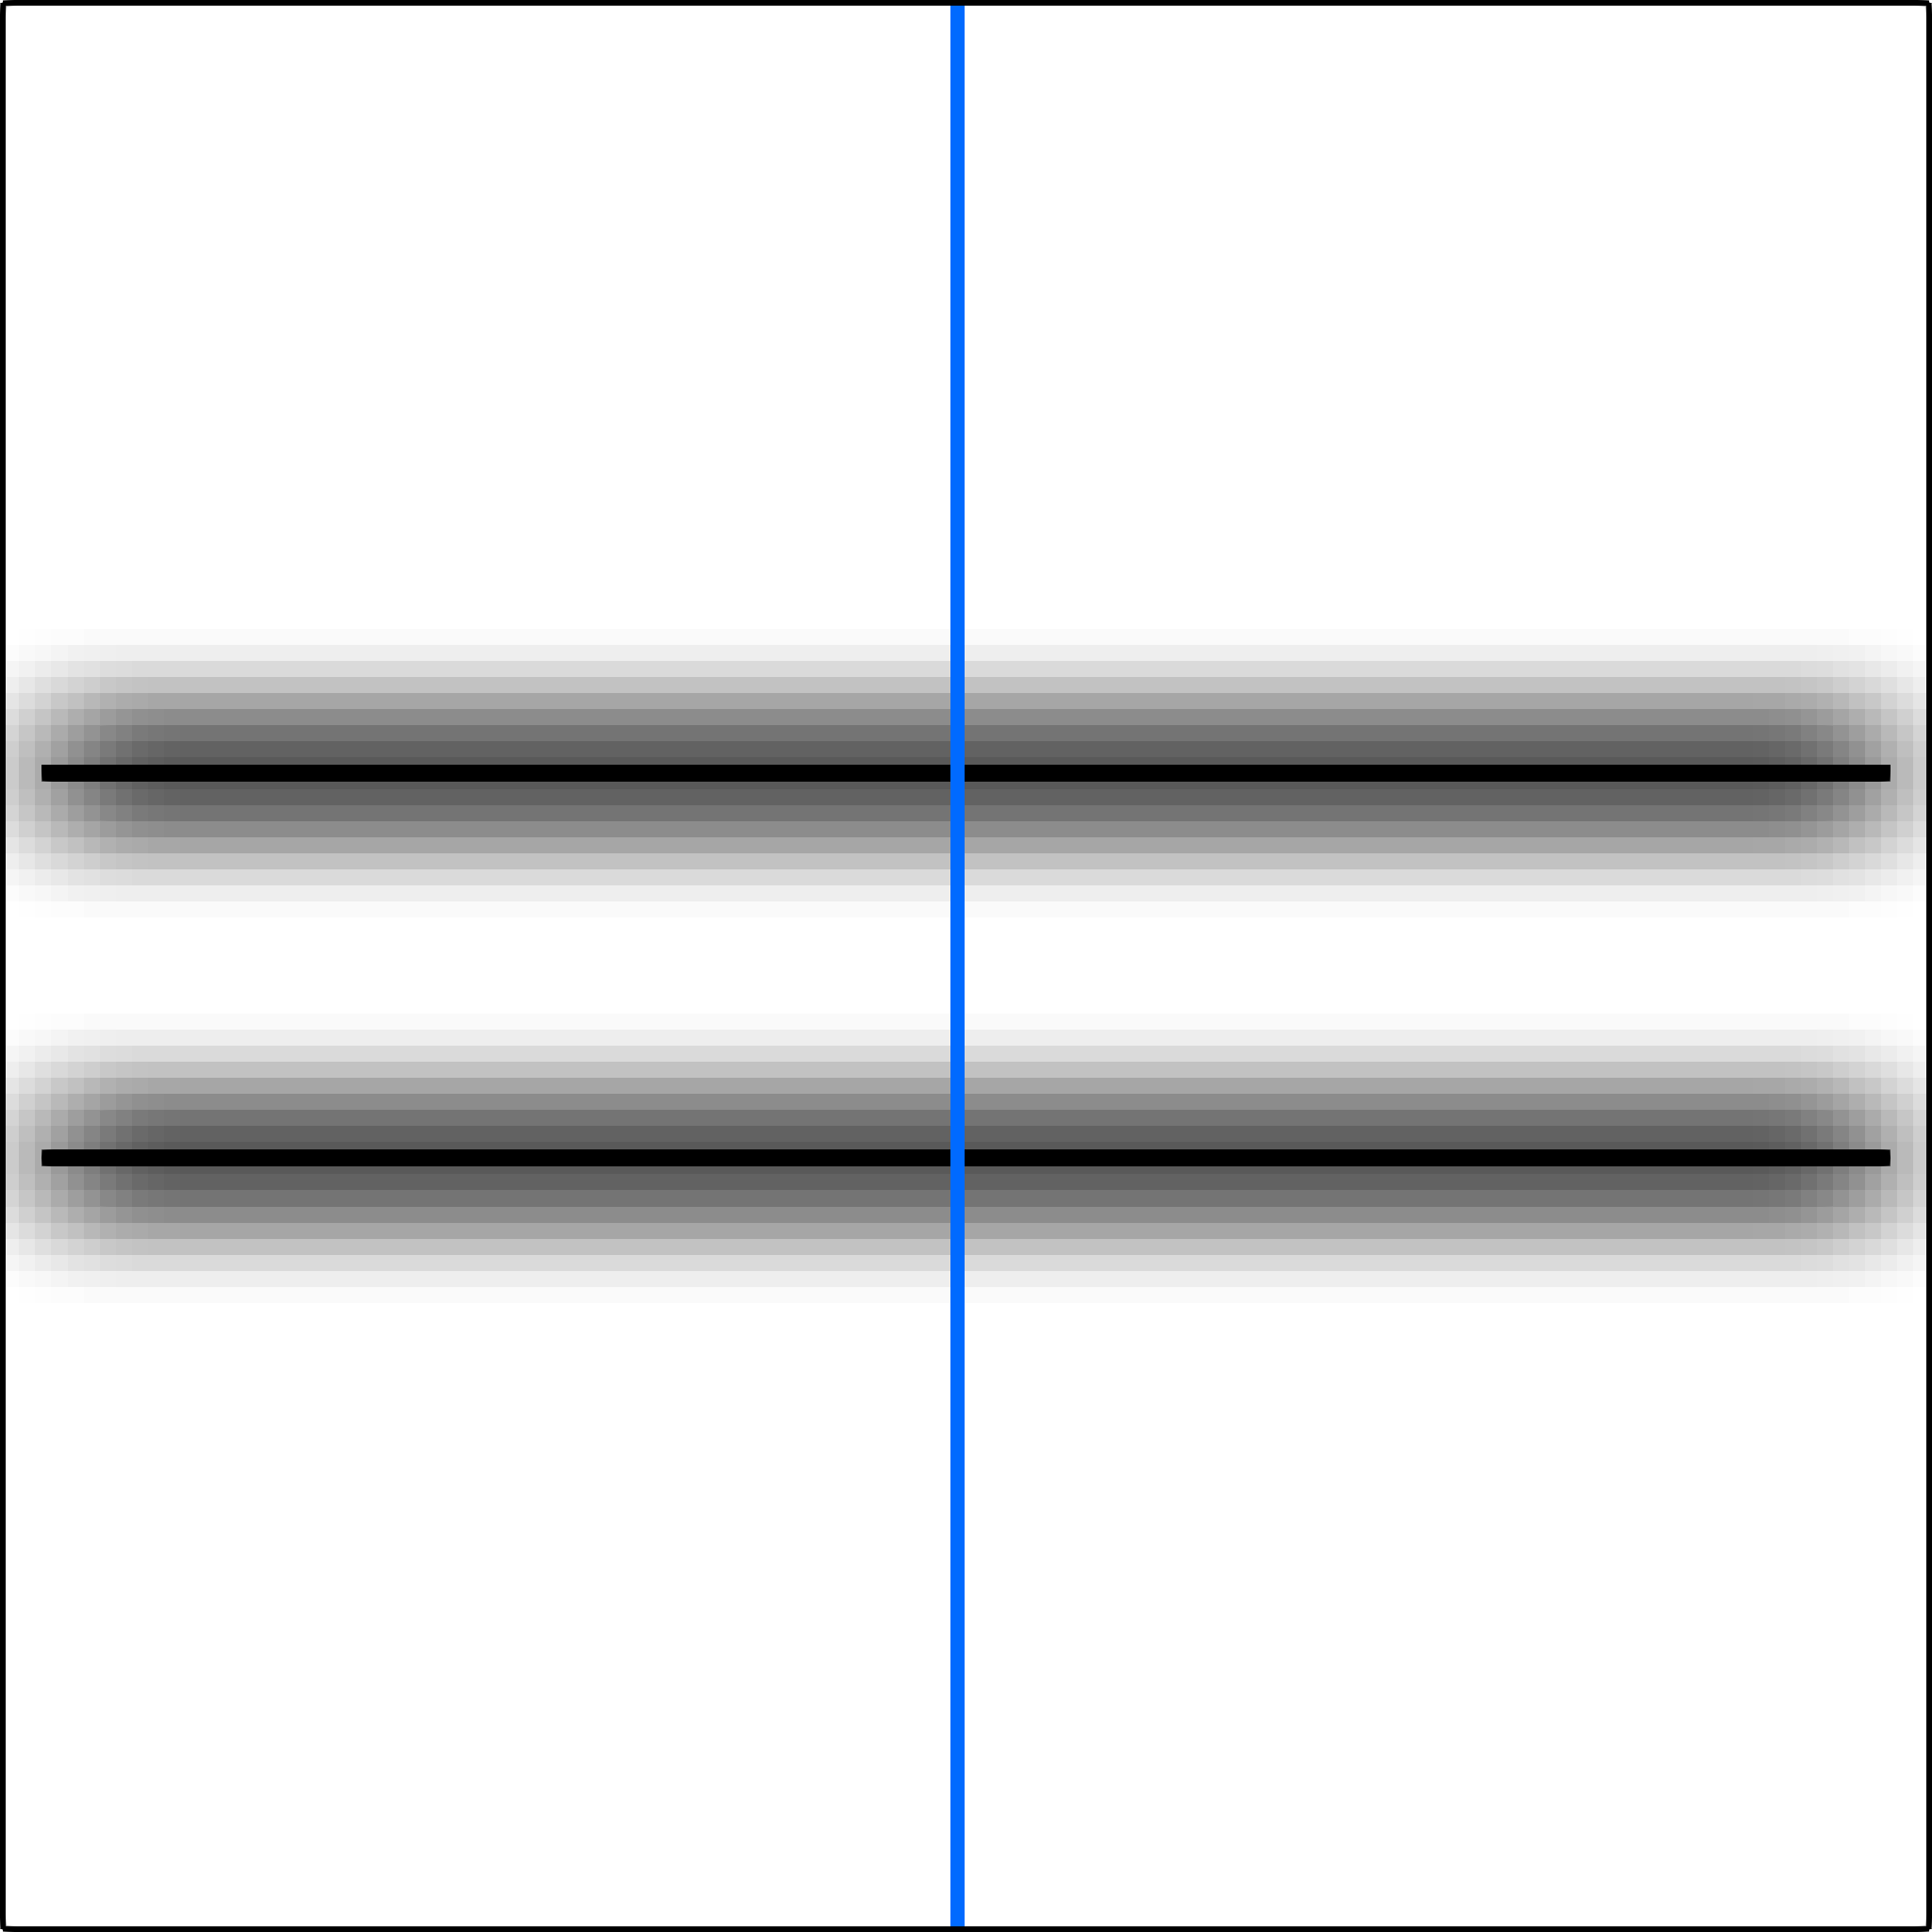
\includegraphics[scale=.075]{figures/FilterRadius/Distant.png}
        \caption*{(a)}
    \end{subfigure}
    \begin{subfigure}{.3\textwidth}
        \centering
        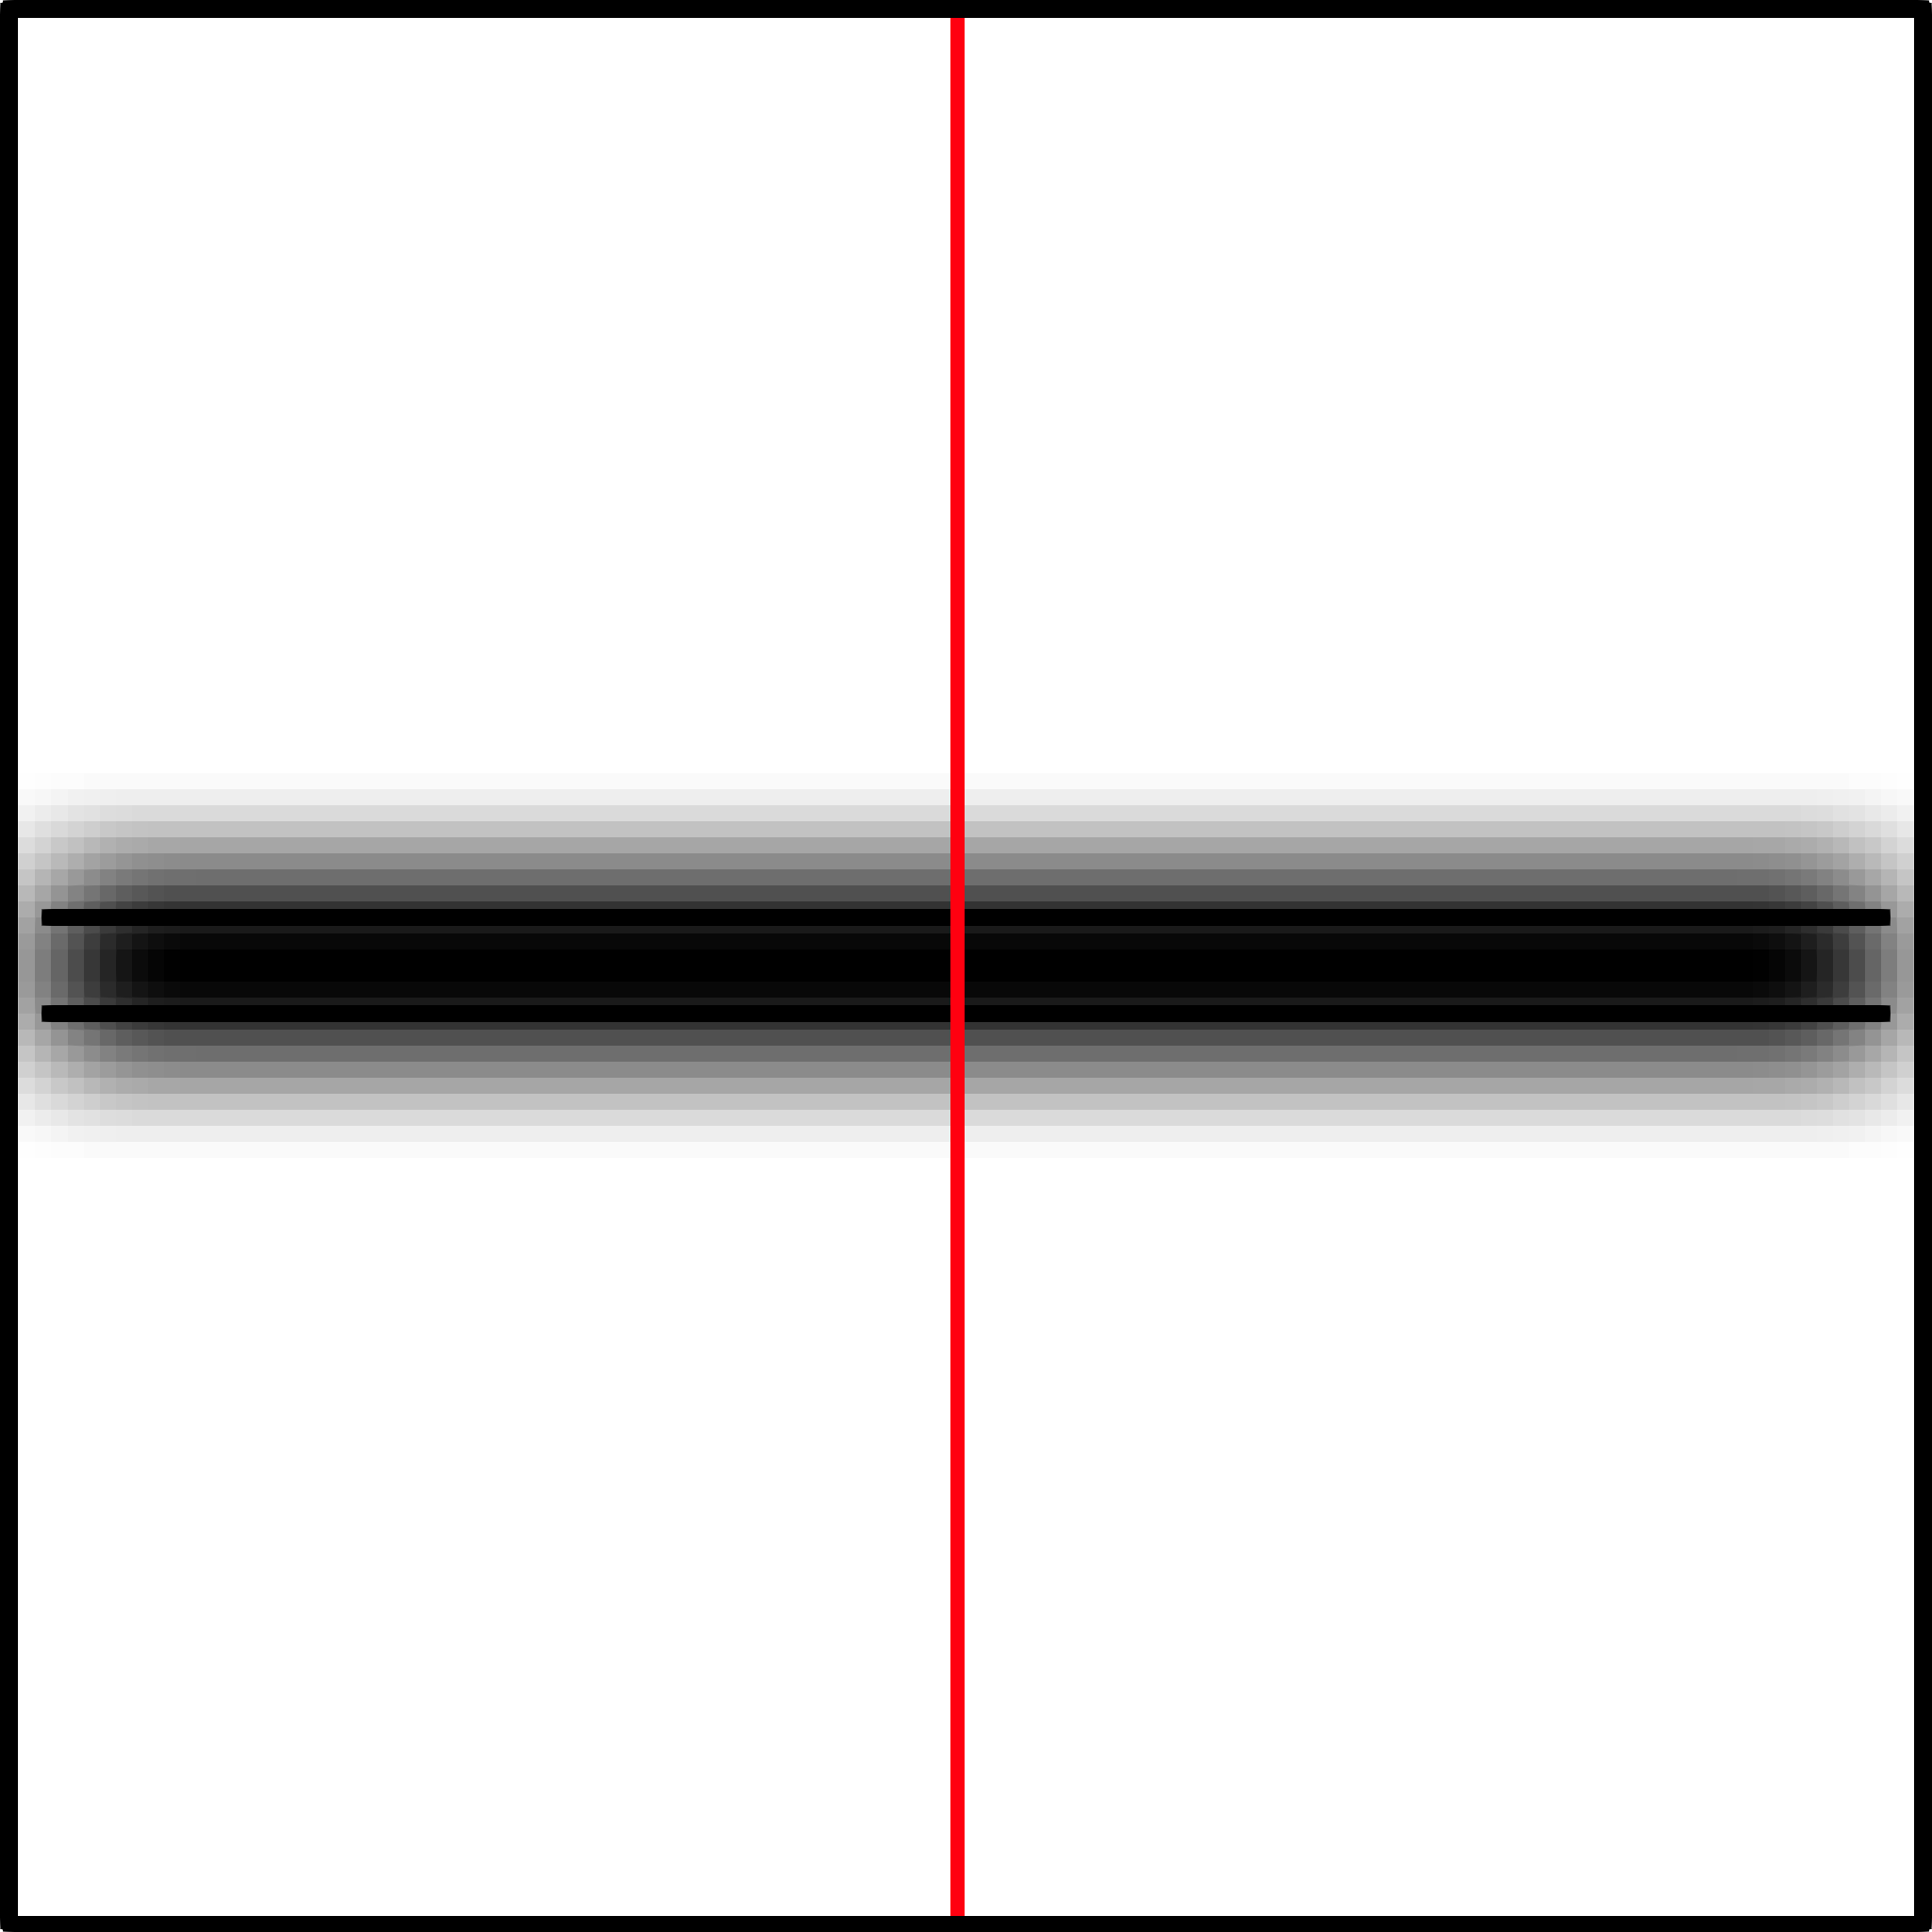
\includegraphics[scale=.075]{figures/FilterRadius/Close.png}
        \caption*{(b)}
    \end{subfigure}
    \begin{subfigure}{.375\textwidth}
        \centering
        \resizebox{\textwidth}{!}{
            % Data for the first, distant pair of horizontal lines. Extracted along the y axis via target.data[20, :].round(3)

% [0.   0.   0.   0.   0.   0.   0.   0.   0.   0.   0.   0.   0.   0.
%  0.   0.   0.   0.   0.   0.   0.   0.   0.   0.   0.   0.   0.   0.
%  0.   0.   0.   0.   0.   0.   0.   0.   0.   0.   0.   0.04 0.11 0.23
%  0.38 0.55 0.71 0.86 0.97 1.03 1.03 0.97 0.86 0.71 0.55 0.38 0.23 0.11
%  0.04 0.   0.   0.   0.   0.   0.   0.04 0.11 0.23 0.38 0.55 0.71 0.86
%  0.97 1.03 1.03 0.97 0.86 0.71 0.55 0.38 0.23 0.11 0.04 0.   0.   0.
%  0.   0.   0.   0.   0.   0.   0.   0.   0.   0.   0.   0.   0.   0.
%  0.   0.   0.   0.   0.   0.   0.   0.   0.   0.   0.   0.   0.   0.
%  0.   0.   0.   0.   0.   0.   0.   0.  ]


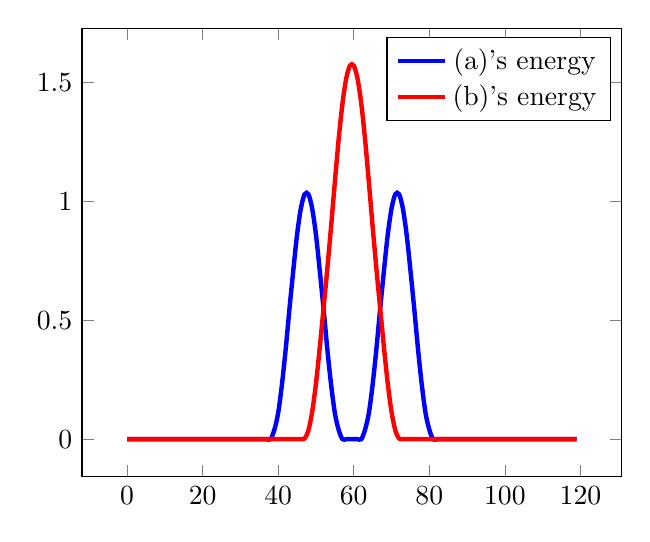
\begin{tikzpicture}
    \begin{axis} [every axis plot post/.append style={ultra thick, mark=none}, xlabel=]
        \addplot +[smooth] [color=blue] coordinates {
            (0, 0.)
            (1, 0.)
            (2, 0.)
            (3, 0.)
            (4, 0.)
            (5, 0.)
            (6, 0.)
            (7, 0.)
            (8, 0.)
            (9, 0.)
            (10, 0.)
            (11, 0.)
            (12, 0.)
            (13, 0.)
            (14, 0.)
            (15, 0.)
            (16, 0.)
            (17, 0.)
            (18, 0.)
            (19, 0.)
            (20, 0.)
            (21, 0.)
            (22, 0.)
            (23, 0.)
            (24, 0.)
            (25, 0.)
            (26, 0.)
            (27, 0.)
            (28, 0.)
            (29, 0.)
            (30, 0.)
            (31, 0.)
            (32, 0.)
            (33, 0.)
            (34, 0.)
            (35, 0.)
            (36, 0.)
            (37, 0.)
            (38, 0.)
            (39, 0.04)
            (40, 0.11)
            (41, 0.23)
            (42, 0.38)
            (43, 0.55)
            (44, 0.71)
            (45, 0.86)
            (46, 0.97)
            (47, 1.03)
            (48, 1.03)
            (49, 0.97)
            (50, 0.86)
            (51, 0.71)
            (52, 0.55)
            (53, 0.38)
            (54, 0.23)
            (55, 0.11)
            (56, 0.04)
            (57, 0.)
            (58, 0.)
            (59, 0.)
            (60, 0.)
            (61, 0.)
            (62, 0.)
            (63, 0.04)
            (64, 0.11)
            (65, 0.23)
            (66, 0.38)
            (67, 0.55)
            (68, 0.71)
            (69, 0.86)
            (70, 0.97)
            (71, 1.03)
            (72, 1.03)
            (73, 0.97)
            (74, 0.86)
            (75, 0.71)
            (76, 0.55)
            (77, 0.38)
            (78, 0.23)
            (79, 0.11)
            (80, 0.04)
            (81, 0.)
            (82, 0.)
            (83, 0.)
            (84, 0.)
            (85, 0.)
            (86, 0.)
            (87, 0.)
            (88, 0.)
            (89, 0.)
            (90, 0.)
            (91, 0.)
            (92, 0.)
            (93, 0.)
            (94, 0.)
            (95, 0.)
            (96, 0.)
            (97, 0.)
            (98, 0.)
            (99, 0.)
            (100, 0.)
            (101, 0.)
            (102, 0.)
            (103, 0.)
            (104, 0.)
            (105, 0.)
            (106, 0.)
            (107, 0.)
            (108, 0.)
            (109, 0.)
            (110, 0.)
            (111, 0.)
            (112, 0.)
            (113, 0.)
            (114, 0.)
            (115, 0.)
            (116, 0.)
            (117, 0.)
            (118, 0.)
            (119, 0.)
        };
        \addplot +[smooth] [color=red] coordinates {
            (0, 0.)
            (1, 0.)
            (2, 0.)
            (3, 0.)
            (4, 0.)
            (5, 0.)
            (6, 0.)
            (7, 0.)
            (8, 0.)
            (9, 0.)
            (10, 0.)
            (11, 0.)
            (12, 0.)
            (13, 0.)
            (14, 0.)
            (15, 0.)
            (16, 0.)
            (17, 0.)
            (18, 0.)
            (19, 0.)
            (20, 0.)
            (21, 0.)
            (22, 0.)
            (23, 0.)
            (24, 0.)
            (25, 0.)
            (26, 0.)
            (27, 0.)
            (28, 0.)
            (29, 0.)
            (30, 0.)
            (31, 0.)
            (32, 0.)
            (33, 0.)
            (34, 0.)
            (35, 0.)
            (36, 0.)
            (37, 0.)
            (38, 0.)
            (39, 0.)
            (40, 0.)
            (41, 0.)
            (42, 0.)
            (43, 0.)
            (44, 0.)
            (45, 0.)
            (46, 0.)
            (47, 0.003)
            (48, 0.037)
            (49, 0.115)
            (50, 0.234)
            (51, 0.384)
            (52, 0.549)
            (53, 0.716)
            (54, 0.894)
            (55, 1.081)
            (56, 1.26)
            (57, 1.41)
            (58, 1.516)
            (59, 1.571)
            (60, 1.571)
            (61, 1.516)
            (62, 1.41)
            (63, 1.26)
            (64, 1.081)
            (65, 0.894)
            (66, 0.716)
            (67, 0.549)
            (68, 0.384)
            (69, 0.234)
            (70, 0.115)
            (71, 0.037)
            (72, 0.003)
            (73, 0.)
            (74, 0.)
            (75, 0.)
            (76, 0.)
            (77, 0.)
            (78, 0.)
            (79, 0.)
            (80, 0.)
            (81, 0.)
            (82, 0.)
            (83, 0.)
            (84, 0.)
            (85, 0.)
            (86, 0.)
            (87, 0.)
            (88, 0.)
            (89, 0.)
            (90, 0.)
            (91, 0.)
            (92, 0.)
            (93, 0.)
            (94, 0.)
            (95, 0.)
            (96, 0.)
            (97, 0.)
            (98, 0.)
            (99, 0.)
            (100, 0.)
            (101, 0.)
            (102, 0.)
            (103, 0.)
            (104, 0.)
            (105, 0.)
            (106, 0.)
            (107, 0.)
            (108, 0.)
            (109, 0.)
            (110, 0.)
            (111, 0.)
            (112, 0.)
            (113, 0.)
            (114, 0.)
            (115, 0.)
            (116, 0.)
            (117, 0.)
            (118, 0.)
            (119, 0.)
        };
        \addlegendentry{(a)'s energy}
        \addlegendentry{(b)'s energy}
    \end{axis}
\end{tikzpicture}
        }
        \caption*{(c)}
    \end{subfigure}
    \caption{
        How the proximity of lines changes the brightness of their respective footprints in a 120x120px image.
        (a): Two lines approx. three times the blur radius apart.
        (b): Two lines only 3/4 the blur radius apart.
        (c): The brightness of the more distant lines (fig. a, blue) and the closer ones (fig. b, red).
        On the x-axis we see the height of the pixels taken along the red and blue strips in (a) and (b) respectively, counted from the top.
    }
    \label[figure]{fig:closeenergy}
\end{figure}
\section{Time Coherence - Definition}
\label[section]{sec:tcdef}
Based on the desired image overlap and concepts from computing the energy measure, we can infer a measure for time coherence.
In fact, we can use a definition analogous to $E$ already defined by Turk and Banks.
To avoid confusion, we will from now on write the spacial components (former $E$ and $L$) as $E_s, L_s$ to better separate them from their temporal counterparts $E_t$ and $L_t$.
Instead of the comparison between a low-pass image of lines and a constant target brightness, the temporal energy $E_t$ now depends on two sets of lines ($I_0, I_1$) and uses a different low-pass filter ($L_t$):
\[E_t(I, I') = \int_x\int_y\left[(L_t\ast I_0)(x,y)-(L_t\ast I_1)(x,y)\right]^2\,dx\,dy\]
This measure would give us the squared difference between the brightnesses of two different sets of lines.
Allowing for a new kernel gives us more freedom to change \textit{how} we measure the temporal energy, as we do not want it to behave the same way as the spatial energy does.
For example, the measure $E_s$ of two neighboring streamlines is the strongest in the center of them, not at the actual line positions, which can be seen in \cref{fig:closeenergy}.
This means that by using $E_s$ instead of $E_t$, we would change the number or position of lines by drawing them into the center of two former lines,
thereby intently worsening time coherence.
Conversely, this would also prohibit streamline creation at darker spots, giving rise to holes in our line image.\\

The optimum for time coherence would of course be two identical sets of streamlines, which effectively minimize $E_t$ to zero.

% Combining it with the spacial measure $E$ via linear interpolation gives us a good amount of control how strong we want the coherence to be.

% Time Coherence refers to how a vector field behaves through different time steps.
% Intuitively, we consider areas within the field to be of high temporal coherence if the lines drawn on them are relatively stationary.
% Vice versa, we can say that an area of high fluctuation will be of low temporal coherence.
% A more formal definition employed in our algorithm is as follows:
% Given a field $F$ and a starting point $S_0$ (called the "seed"), we can integrate over the field.
% This yields a set of points $S^0$ which define a streamline containing every reached point, written as $S^0 = \int(S_0, F)$.
% We can therefore assign a streamline to every point in our field (and vice versa).
% Given $S_0$ and an unsteady field $F(t)$, compute for each time step $t_1...t_n$ the streamline $S^{0,t_i} = \int(S_0, F(t_i))$.
% In order to convert these sets of lines to a scalar, we use the Hausdorff Distance $dist(S^i,S^j)$,
% giving us the greatest minimal distance between any pair of two sets.
% We can therefore create a map $coh(S_i, F(t)): max(dist(\int(S_i, F(t_k)), \int(S_i, F(t_l))))$,
% sending each point in an unsteady vector field to a scalar, and thereby determining its temporal coherence.
